% LaTeX Template for short student reports.
% Citations should be in bibtex format and go in references.bib
\documentclass[a4paper, 11pt]{article}
\usepackage[top=3cm, bottom=3cm, left = 2cm, right = 2cm]{geometry} 
\geometry{a4paper} 
\usepackage[utf8]{inputenc}
\usepackage{textcomp}
\usepackage{graphicx} 
\usepackage{amsmath,amssymb}  
\usepackage{bm}  
\usepackage[pdftex,bookmarks,colorlinks,breaklinks]{hyperref}  


\documentclass{article}
\usepackage{listings}
\usepackage{xcolor}

\definecolor{codegreen}{rgb}{0,0.6,0}
\definecolor{codegray}{rgb}{0.5,0.5,0.5}
\definecolor{codepurple}{rgb}{0.58,0,0.82}
\definecolor{backcolour}{rgb}{0.95,0.95,0.92}

\lstdefinestyle{mystyle}{
    backgroundcolor=\color{backcolour},   
    commentstyle=\color{codegreen},
    keywordstyle=\color{magenta},
    numberstyle=\tiny\color{codegray},
    stringstyle=\color{codepurple},
    basicstyle=\ttfamily\footnotesize,
    breakatwhitespace=false,         
    breaklines=true,                 
    captionpos=b,                    
    keepspaces=true,                 
    numbers=left,                    
    numbersep=5pt,                  
    showspaces=false,                
    showstringspaces=false,
    showtabs=false,                  
    tabsize=2
}
%\hypersetup{linkcolor=black,citecolor=black,filecolor=black,urlcolor=black} % black links, for printed output
\usepackage{memhfixc} 
\usepackage{pdfsync}  
\usepackage{fancyhdr}
\usepackage{mathpazo}
\pagestyle{fancy}

\title{COMP6257 Coursework 1}
\author{Frederik McArthur, fsm1g19@soton.ac.uk}
%\date{}

\begin{document}
\maketitle
\tableofcontents

\section{Introduction}
\label{section:partitionedmatrix}

My project was about \ldots

I developed a system to \ldots

We did some experiments to find out \ldots

The main results were \ldots

\pagebreak

\section{Verifying the Inverse of a Partitioned Matrix}

The inverse of a partitioned matrix is given by:
$$
\begin{bmatrix}
    A & B \\
    C & D
\end{bmatrix}^{-1}
= \begin{bmatrix}
    M & -MBD^{-1} \\
    -D^{-1}CM & D^{-1} + D^{-1}CMBD^{-1}
\end{bmatrix}
    $$
Where $M = \begin{bmatrix}
    A - BD^{-1}C
\end{bmatrix}^{-1}$. To verify that $\begin{bmatrix}
    M & -MBD^{-1} \\
    -D^{-1}CM & D^{-1} + D^{-1}CMBD^{-1}
\end{bmatrix}$ is the inverse of $\begin{bmatrix}
    A & B \\
    C & D
\end{bmatrix}$, the following condition must be met:
$$
\begin{bmatrix}
    A & B \\
    C & D
\end{bmatrix} * 
\begin{bmatrix}
    M & -MBD^{-1} \\
    -D^{-1}CM & D^{-1} + D^{-1}CMBD^{-1}
\end{bmatrix}
= \begin{bmatrix}
    I & 0 \\
    0 & I
\end{bmatrix}$$
Examining each element of the matrix, and using the knowledge that $A*I = I*A = A$, and $A*A^{-1} = A^{-1}A = I$;
\begin{itemize}
    \item Row 1 Column 1;
    \begin{align*}
        AM + B(-D^{-1}CM) &= I\\
        AM - BD^{-1}CM &= I\\
        M * (A - BD^{-1}C) &= I\\
        M * M^{-1} &= I
    \end{align*}
    \item Row 1 Column 2;
    \begin{align*}
        A (-MBD^{-1}) + B(D^{-1} + D^{-1}CMBD^{-1}) &= 0 \\
        -AMBD^{-1} +BD^{-1} + BD^{-1}CMBD^{-1} &= 0\\
        (AM + I + BD^{-1}CM)BD^{-1} &= 0\\
        ((A-BD^{-1}C)M - I)BD^{-1} &= 0 \\
        (M^{-1}M - I)BD^{-1} &= 0 \\
        (I - I) BD^{-1} &= 0
    \end{align*}
    \item Row 2 Column 1;
    \begin{align*}
        CM + D(-D^{-1}CM) &= 0 \\
        CM - DD^{-1}CM &= 0 \\
        CM - ICM &= 0\\
        CM - CM &= 0
    \end{align*}
    \item and finally, Row 2 Column 2;
    \begin{align*}
        C(-MBD^{-1}) + D(D^{-1} + D^{-1}CMBD^{-1}) &= I \\
        -CMBD^{-1} +  DD^{-1} + DD^{-1}CMBD^{-1} &= I \\
        -CMBD^{-1} + I + ICMBD^{-1} &= I \\
        -CMBD^{-1} + CMBD^{-1} + I &= I \\
        I &= I
    \end{align*}
\end{itemize}
This demonstrates that $
\begin{bmatrix}
    A & B \\
    C & D
\end{bmatrix}^{-1}
= \begin{bmatrix}
    M & -MBD^{-1} \\
    -D^{-1}CM & D^{-1} + D^{-1}CMBD^{-1}
\end{bmatrix}
    $.


    
\pagebreak

\section{Inverse of a rank one update of a matrix}

To demonstrate that a matrix is the inverse, as demonstrated in Section \ref{section:partitionedmatrix}, the $A*I = I*A = A$ identity can be used to prove this. Therefore, when examining 

$$ [A + xx^T ]^{-1} = A^{-1} - \frac{A^{-1}xx^TA^{-1}}{1 + x^TA^{-1}x}$$

we can prove that $\frac{A^{-1}xx^TA^{-1}}{1 + x^TA^{-1}x}$ is the inverse by the following process;

\begin{align*}
    I &= [A + xx^T ] \left(A^{-1} - \frac{A^{-1}xx^TA^{-1}}{1 + x^TA^{-1}x}\right) \\
    I &= AA^{-1} + xx^TA^{-1} - \frac{AA^{-1}xx^TA^{-1} + xx^TA^{-1}xx^TA^{-1}}{1 + x^TA^{-1}x}\\
    I &= I + xx^TA^{-1} - \frac{xx^TA^{-1} + xx^TA^{-1}xx^TA^{-1}}{1+x^TA^{-1}x} \\
    I &= I + xx^TA^{-1} - \frac{x(1+x^TA^{-1}x)x^TA}{1+x^TA^{-1}x} \\
    I &= I + xx^TA^{-1} - xx^TA^{-1} \\
    I &= I
\end{align*}
 Thus, proving that the inverse of a Rank one update of a matrix is given by 
$$ [A + xx^T ]^{-1} = A^{-1} - \frac{A^{-1}xx^TA^{-1}}{1 + x^TA^{-1}x}$$

\section{Bayesian Estimation}

Equations 2.141 (Equation \ref{eq:prml2141}) and 2.142 (Equation \ref{eq:prml2142}) in Pattern Recognition and Machine Learning are given as follows:

\begin{equation} \label{eq:prml2141}
\mu_N = \frac{\sigma^2}{N\sigma_0^2 + \sigma^2}\sigma_0 + \frac{N\sigma^2}{N\sigma_0^2 + \sigma^2}\sigma_{ML}
\end{equation}

\begin{equation} \label{eq:prml2142}
\frac{1}{\sigma^2_N} = \frac{1}{\sigma^2_0} + \frac{N}{\sigma^2}
\end{equation}

\subsection{When $N \rightarrow \infty$}

When $N$ tends towards infinity, Equation \ref{eq:prml2141} will tend towards the maximum likelihood solution, as $\frac{\sigma^2}{N\sigma_0^2 + \sigma^2}$ will tend towards zero, leaving $\mu_N = \frac{N\sigma^2}{N\sigma_0^2 + \sigma^2}\sigma_{ML}$. 
Similarly, in Equation \ref{eq:prml2141}, the variance will tend towards zero, as the right hand side of the equation will tend towards infinity, and $\frac{1}{\infty} \rightarrow 0$.

\subsection{A highly confident Prior}

For a highly confident prior, the variance would tend towards zero, so $\sigma_0 \rightarrow 0$. This would mean that the mean would reduce to the prior value, and not the maximum likelihood value. 

\section{Bayesian Analysis of the Illustrative Polynomial}

The dataset generated for this problem was generated with Numpy, first by generating a uniform dataset, and then by applying a sinusoidal function to it. The Sklearn \verb|train_test_split| function is then used to split the dataset into both a training and a testing dataset. A plot of the training and testing dataset can be seen in Figure \ref{fig:traintestsplit}.

\begin{figure}[h]
    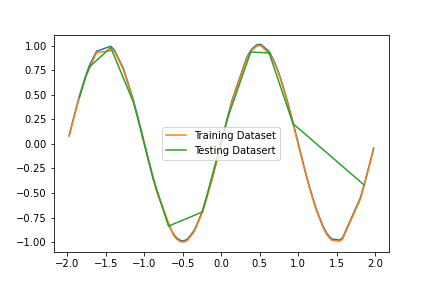
\includegraphics[width=8cm]{fig/traintestsplit.png}
    \caption{A figure showing the training and testing datasets.}
    \label{fig:traintestsplit}
\end{figure}

Polynomial regression was then performed on the data, with trials at different P values. As shown in Figure \ref{fig:pvalueboxplt} shows that as the P value increases, the accuracy increases towards a point. Beyond a certain value, the graph will begin to over fit.

\begin{figure}[h]
    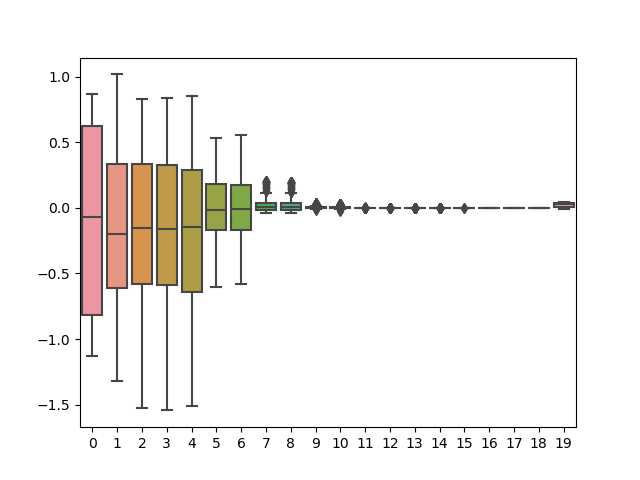
\includegraphics[width=8cm]{fig/pvalueboxplot.png}
    \caption{A figure showing the error values for different p values.}
    \label{fig:traintestsplit}
\end{figure}

\pagebreak

\section{Robot Navigation Problem}

For the sampling problems, I created a mixture distribution from the equations provided in the coursework. These distributions were defined as:



\begin{equation}\label{eq:gauss1}
        p_1(x) &= \mathcal{N}(x|\mu_1, \sigma_1) \: where \: \mu_1 = \begin{bmatrix}2.0 \ 5.0\end{bmatrix}, \sigma_1 = \begin{bmatrix}2 & 1 \ 1 & 2\end{bmatrix} \\
        p_2(x) &= \mathcal{N}(x|\mu_2, \sigma_2) \: where \: \mu_2 = \begin{bmatrix}3.0 \ 1.0\end{bmatrix}, \sigma_2 = \begin{bmatrix}0.1 & 0 \ 0 & 0.1\end{bmatrix} = 0.1 \mathcal{I} \\
        p(x) &= p_1(x) + p_2(x)
\end{equation}

with the mixture distributions defined as $ p(x) = p_1(x) + p_2(x)$. 

I also created a distribution for use in both Rejection and Importance sampling, defined as 


\begin{equation}\label{eq:dist}
        q(x) = \mathcal{N}(x|\mu_q, \sigma_q) \: where \: \mu_q = \begin{bmatrix}2.5 \ 4.0\end{bmatrix}, \sigma_q = \begin{bmatrix}3 & 0.2 \ 0.3 & 4\end{bmatrix}
\end{equation}
where the two distributions were enclosed as much as reasonably possible. These distributions are visible in Figure \ref*{fig:distributions}.

\begin{figure}[h]
    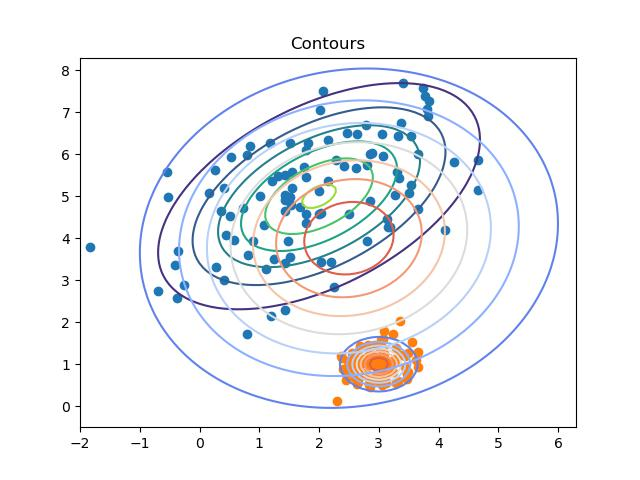
\includegraphics[width=8cm]{fig/distributionsplotted.jpg}
    \caption{A figure showing distribution 1, 2 and the enclosing normal distribution. Distribution $p_1$ is the oval shaped distribution in the top left, and distribution $p_2$ is the small distribution in the bottom right. Distribution 3 is the enclosing distribution.}
    \label{fig:distributions}
\end{figure}

\subsection{Rejection Sampling}

\begin{figure}[h]
    
\includegraphics[width=8cm]{fig/3dcontour.jpg}
    \caption{A figure showing the three contours, and plots of the samples which were calculated in the Rejection sampling processs. Points in orange are rejected, and points in blue are accepted. The sample size is $n=100$}
    \label{fig:rejectionsampling}
\end{figure}
To perform rejection sampling, the normal distribution shown in Equation \ref{eq:dist} is created for a set number of samples. Each sample is then iterated over, with the probability of the mixed distribution calculated. If the combined probability is less than the probability of the q distribution, then the sample value is accepted.

The output of the Rejection sampling algorithm can be seen in Figure \ref*{fig:rejectionsampling}.



The code for the rejection sampling can be found below:
\begin{lstlisting}[language=Python, caption=Rejection Sampling Code.]
def rejection(q_mean, q_var, q, k, dist1, dist2, w, n = 1000, 
    forced_input = False, forced_input_value = None):

    #   Defining the varibles for accepted and rejected variables.
    accepted, u_accepted, rejected, u_rejected = [],[],[],[] 

    #   Creating the samples from the provided distribution information.
    samples = np.random.multivariate_normal(q_mean, q_var, n)

    #   If the input is forced, set the samples to be the input. Used for 
    # calculating the probability for a specific value.
    if forced_input:
    samples = forced_input_value

    #   Iterating over the samples.
    for sample in samples:
    #   Calculating the mixed gaussian probability dist,
    # with the weights.
    prob_dist_1 = w[0]*dist1(sample)
    prob_dist_2 = w[1]*dist2(sample)
    combined_prob = prob_dist_1 + prob_dist_2

    u_bound = k * q(sample)

    u = u_bound #np.random.uniform(low = 0, high=u_bound)

    #   If the combined prob is less than the q dist prob
    if combined_prob > u:
    # Accept result
    accepted.append(sample)
    u_accepted.append(u)
    else:
    # else, reject the result
    rejected.append(sample)
    u_rejected.append(u)

    # Return an array of results.
    return np.array(accepted),np.array(u_accepted), np.array(rejected), np.array(u_rejected)
\end{lstlisting}

\subsection*{Importance Sampling}

Importance sampling was performed by calculating the following value:

\begin{equation}\label{eq:importance}
        \mathcal{E}[x] = \frac{1}{n} \sum_{i=0}^n x_i \frac{p(x_i)}{q(x_i)} q(x_i)
\end{equation}

Where $\frac{p(x_i)}{q(x_i)} q(x_i)$ are the importance weights of the problem. 

This calculation prpvodes the probability of the selection of the value in the mixture distribution defined in Equation \ref*{eq:gauss1}. The code for this can be found below:
\begin{lstlisting}[language=Python, caption=Importance Sampling Code.]
    def importance(q, w, dist1, dist2, vals):
        #   Calculate the weights from the distributions
        weights = ((w[0] * dist1(vals)) + (w[1] * dist2(vals))) / q(vals) #np.sum(((w[0] * dist1(samples)) + (w[1] * dist2(samples))))
        weights = weights * q(vals)

        #   Calculate the probability by multiplying by the weights.
        y = np.sum(weights*vals)/len(vals)

        #   Return the probability.
        return y
\end{lstlisting}

\subsection*{Comparison between results}

Examining the point $x = [4.0, 4.0]^T$, importance sampling and rejection sampling score similarly. Importance sampling produces a probability of $p_i = 0.032078$, where rejection sampling produces a probability of $p_r = 0.031606$. These probabilities are very similar, with each algorithm rejecting the position. 
\pagebreak

\section{Conclusions and Future Work}

From our experiments we can conclude that \ldots

\bibliographystyle{abbrv}
% \bibliography{references}  % need to put bibtex references in references.bib 
\end{document}